\documentclass{article}

% Language setting
% Replace `english' with e.g. `spanish' to change the document language
\usepackage[english]{babel}

% Set page size and margins
% Replace `letterpaper' with `a4paper' for UK/EU standard size
\usepackage[a4paper,top=2cm,bottom=2cm,left=3cm,right=3cm,marginparwidth=1.75cm]{geometry}

% Useful packages
\usepackage{amsmath}
\usepackage{graphicx}
\usepackage[colorlinks=true, allcolors=blue]{hyperref}
\usepackage{cleveref}

\title{Scribbles on the problem}
\author{Amazing group}

\begin{document}
\maketitle

\begin{abstract}
We are trying hard to use the data to optimise those paths
\end{abstract}

\section{Introduction}

An aeroplane is only able to maintain itself flying if the lift is at least equal to its weight. That means, for a plane flying in a horizontal direction, with no change in altitude, we have:
%
\begin{equation}
    \notag
    m(t) g = \frac{1}{2} C_L(\theta) S_{W} \rho U^2
\end{equation}
%
where $m(t)$ is the mass of the plane, $g$ is the gravitational acceleration, $C_L$ is the lift coefficient, which depends on the angle of attack $\theta$, $S_W$ is the cross-sectional area of the wings, $\rho$ is the density of air, and $U$ is the speed of the airplane relative to wind. It is important to remember that the change in mass due to fuel consumption is significative throughout the flight: "Airliners have a fuel fraction of less than half their takeoff weight, between 26\% for medium-haul to 45\% for long-haul." \href{https://en.wikipedia.org/wiki/Fuel_fraction}{Wikipedia}. 

Also, if the airplane maintains a constant velocity with respect to the ground, we have that the thrust force from the engine is given by
%
\begin{equation}
    \notag
    T = D + m(t)g \sin(\gamma),
\end{equation}
%
where $D$ is the drag force and $\gamma$ is the pitch angle. Assuming the pitch angle is very small, a good approximation is $\sin{\gamma} \approx \gamma$.

\section{Simple metrics for time, distance and fuel consumption}

\subsection{Time}

Time is the most reliable and simple calculation given data from any plane. The metric is final time minus initial time $\Delta t = t_f - t_i$.

\subsection{Distance}

Distance can be a bit trickier, we need to compute a discretisation of the line integral of distance over the trajectory:
%
\begin{equation}
    \Delta s = \int_{t_i}^{t_f} |\vec{v}_g(t)| \mathrm d t.
\end{equation}

\subsection{Fuel consumption}
\label{subsec:fuel}

A typical curve of fuel consumption is shown in \Cref{fig:fuel-consumption} below. We are interested in the middle region, not including take-off and landing.
%
\begin{figure}
    \centering
    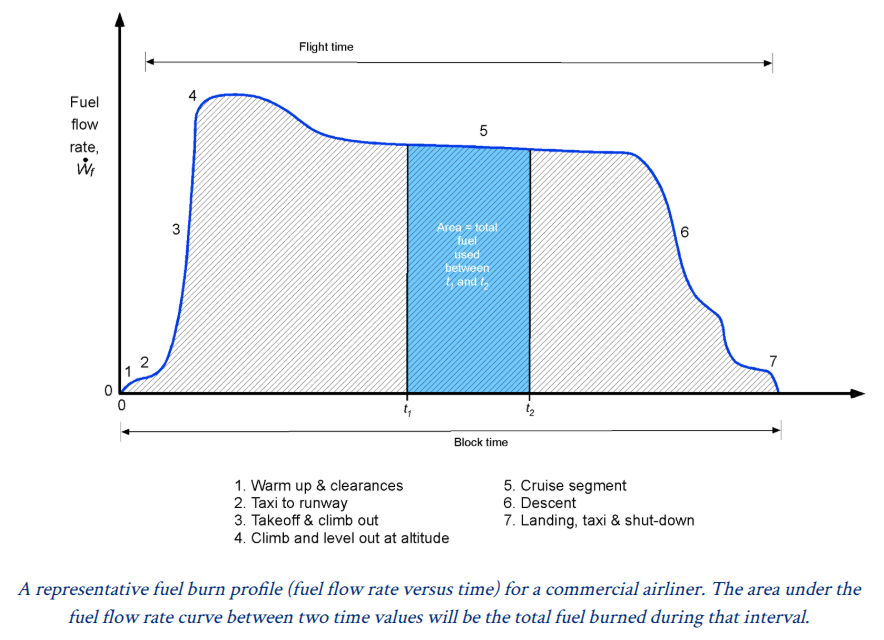
\includegraphics[width=0.85\linewidth]{Screenshot from 2025-07-15 11-41-21.png}
    \caption{Taken from \href{https://eaglepubs.erau.edu/introductiontoaerospaceflightvehicles/chapter/flight-range-endurance/}{Embry-Riddle Aeronautical University}}
    \label{fig:fuel-consumption}
\end{figure}
%
In this region, we expect as little acceleration as possible, so we can assume the thrust is only balancing weight and drag.

We can have a lower bound on fuel consumption if we assume thrust equals drag force throughout the flight. That means:
%
\begin{equation}
    \notag
    T = D = \frac{1}{2} C_D S_{P} \rho U^2,
\end{equation}
%
where $C_D$ is the drag coefficient and $S_P$ is the cross section area of the plane. If we assume the surface area $S_P$ does not change much throughout the flight, we have an estimate for fuel consumption due to drag.
%
\begin{equation}
    \Delta f_D \propto \int_{t_i}^{t_f} T \mathrm d t \propto \int_{t_i}^{t_f} \rho U^2 \mathrm d t.
\end{equation}
%

About the fuel consumption due to acceleration, there is a simple metric to account for accumulated acceleration:
%
\begin{equation}
    \Delta f_a = \int_{t_i}^{t_f} \left| \frac{d \vec{v}}{d t} \right| \mathrm d t.
\end{equation}

\bibliographystyle{alpha}
\bibliography{sample}

\end{document}
